\documentclass[addpoints]{exam}

\usepackage{graphicx}
\usepackage{hyperref}
\usepackage{tabularx}

% Header and footer.
\pagestyle{headandfoot}
\runningheadrule
\runningfootrule
\runningheader{CS 440 CG}{HW 4 Transformations}{Fall 2019}
\runningfooter{}{Page \thepage\ of \numpages}{}
\firstpageheader{}{}{}

\qformat{{\large\bf \thequestion. \thequestiontitle}\hfill}
% \qformat{{\large\bf \thequestion. \thequestiontitle}\hfill[\totalpoints\ points]}
\boxedpoints
% \printanswers

\title{Homework 4: Transformations}
\author{CS 440 Computer Graphics\\Habib University\\Fall 2019}
\date{Due: 18h on Mon, 21 Oct}
% \date{\numpoints\ points and \numbonuspoints\ bonus points, Due: 5p.m. on Mar 4}

\begin{document}
\maketitle
\thispagestyle{empty}

Each problem below specifies the names of the files you have to submit for it. Please make sure your submitted files have the indicated names. Any files in your GitHub repository with these names at the time of the deadline will be considered as your submission.

For interactive programs, the interactive controls should be clearly visible or specified on the page. No modification in the JS file should be necessary.

\begin{questions}
  \titledquestion{Meshes}

  \begin{tabularx}{\linewidth}{lX}
    \raisebox{-.95\totalheight}{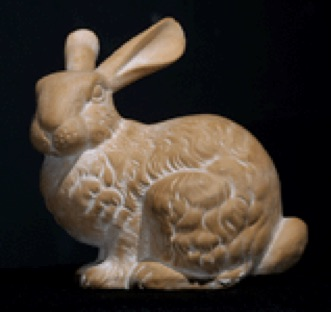
\includegraphics[width=.3\textwidth]{bunny}}
    &
  Browse the \href{http://graphics.stanford.edu/data/3Dscanrep/}{The Stanford 3D Scanning Repository} and download any (or all!) of the 3D models. Write a program to load a mesh from file and transform it to WebGL's default clip coordinates such that the aspect ratio of the model is preserved and the model is centered at the origin.
The program should provide the user the means to interact in the following ways with the model.
\end{tabularx}
  \begin{parts}
    \part Rotate the model slightly about each of the 3 axes in the clockwise or counterclockwise direction.
    \part Shift the model slightly in the positive and negative x, y, or z directions.
    \part Shrink or grow the model slightly along any of the x, y, or z directions.
    \part Reflect the model about any of the axes.
    \part Apply a positive or negative shear to the model along any of the axes.
    \part Reset all transformations.
  \end{parts}
  
  Your JS will have to read the mesh file saved locally. Declare a global variable to save the name of the local file. You can read a local file in JS by \href{https://stackoverflow.com/a/46129280/1382487}{using the fetch API}. Browsers usually do not allow JS to load a local file for security purposes, so you have to make some modifications to enable this behavior.
  \begin{itemize}
  \item On Safari, click on \href{https://stackoverflow.com/questions/4556429/disabling-same-origin-policy-in-safari}{\tt Develop -> Disable Cross-Origin Restrictions}.
  \item On Chrome, set up a web server through the \href{https://chrome.google.com/webstore/detail/web-server-for-chrome/ofhbbkphhbklhfoeikjpcbhemlocgigb}{Web Server for Chrome} browser extension and set as web server the folder containing your files.
  \item On Firefox, there seems to be no restriction!
  \end{itemize}
  \noindent\underline{Files}: {\tt mesh.html, mesh.js}

\end{questions}

\end{document}